\documentclass[titlepage,a4paper,12pt,thmsb]{report}
%%%%%%%%%%%%%%%%%%%%%%%%%%%%%%%%%%%%%%%%%%%%%%%%%%%%%%%%%%%%%%%%%%%%%%%%%%%%%%%%%%%%%%%%%%%%%%%%%%%%%%%%%%%%%%%%%%%%%%%%%%%%
\usepackage{graphicx}
\usepackage{graphics}
\usepackage[english]{babel}
\usepackage[left=1.5in, right=1.5in, top=1in, bottom=1in]{geometry}
\usepackage{float,epsfig,floatflt}
\usepackage{amsmath, amssymb}
\usepackage{a4}
\usepackage[nottoc]{tocbibind}
\usepackage{siunitx}
\usepackage{fancyhdr}
\usepackage{makeidx}
\usepackage{multirow}
\usepackage[most]{tcolorbox}
\usepackage{moreverb}
%\usepackage{loremipsum}
\usepackage{tabularx}
\usepackage{tabulary}
\usepackage{subcaption}
\usepackage{multirow}
\usepackage{ragged2e}
\justifying
\usepackage{booktabs}
\usepackage{caption}
\usepackage{textcomp}
\usepackage{multirow}
% \usepackage{amsthm,amsmath}
\usepackage{newtxtext,newtxmath}
\usepackage{caption}
\usepackage{xcolor}
% \usepackage{subcaption}
\usepackage[ruled,linesnumbered]{algorithm2e}
\usepackage{enumitem}
\usepackage[most]{tcolorbox}
\usepackage{balance}
\usepackage{url}
\usepackage{pifont} % Include the pifont package
\usepackage{tabularx}
\usepackage{graphicx}
\usepackage{array}
\usepackage{longtable}
\usepackage{amsmath,amsfonts}
\usepackage{array}
\usepackage{algorithmic}
\usepackage{tocloft}
\usepackage{graphicx}
\usepackage{textcomp}
\usepackage{xcolor}
\usepackage{float}
\usepackage{booktabs}
\usepackage{subcaption}
\usepackage{multirow}
\usepackage{enumitem}
\usepackage{tabularx}
\usepackage{adjustbox}
\usepackage[most]{tcolorbox}
\usepackage{balance}
\usepackage[colorlinks, linkcolor=black, citecolor=blue]{hyperref}
\usepackage{listings}
\usepackage{tipa}
\usepackage{svg}
\usepackage{color, colortbl}
\usepackage{soul}
\usepackage{fancyhdr}
\usepackage{subfloat}
\usepackage[skip=1pt,labelfont=bf]{caption}
\usepackage{marginnote}
\usepackage[colorinlistoftodos]{todonotes}
\usepackage{cancel}
\usepackage{ragged2e}
\usepackage{threeparttable}

\SetAlCapFnt{\small}
\SetAlCapNameFnt{\small}
\usepackage{algorithmic}
\algsetup{linenosize=\small}
\SetKwInput{KwInput}{Input}                % Set the Input
\SetKwInput{KwOutput}{Output}              % set the Output

% \textwidth 16cm \textheight 22.5cm \selectlanguage{english}
% \topmargin 0cm \headheight 0.5 cm \oddsidemargin 0cm
% \evensidemargin 0cm
\renewcommand{\baselinestretch} {1.2} \setlength{\parindent}{0.0cm}
\setlength{\parskip} {0.5 cm}
%\renewcommand{\thesection}{\arabic{section}}
\renewcommand{\thechapter}{\arabic{chapter}}
\setcounter {secnumdepth}{5} \setcounter{tocdepth}{5}
\let\oldTitle\title
\renewcommand{\title}[1]{\newcommand{\myTitle}{#1}\oldTitle{#1}}
\newcommand{\leftscripts}[3]{{\vphantom{#3}}^{#1}_{#2}{#3}}


\newtcolorbox{boxA}{
    boxrule = 1.5pt,
    % rounded corners,
    colback = myblue, % background color
    boxsep=0.1pt,
    top=3pt,bottom=2pt,
    boxrule=1pt,
    frame hidden,
    sharp corners,
    enhanced,
    borderline north={1pt}{0pt}{black},
    borderline south={1pt}{0pt}{black},
    boxsep=2pt,left=2pt,right=2pt,top=2.5pt,bottom=2pt
}
% \definecolor{mygrey}{HTML}{d3d3d3}
\definecolor{myblue}{HTML}{F5DDFE}
% \definecolor{mygreen}{HTML}{CEF5D3}
\definecolor{mygreen}{rgb}{0,0.6,0}
\definecolor{mygray}{rgb}{0.5,0.5,0.5}
\definecolor{mymauve}{rgb}{0.58,0,0.82}
\lstset{
 backgroundcolor=\color{white}, 
 basicstyle = \footnotesize \ttfamily,       
 breakatwhitespace = false,        
 breaklines = true,                 
 captionpos = b,                    
 commentstyle = \color{mygreen}\bfseries,
 extendedchars = false,             
 % frame =shadowbox, 
 frame=leftline,
 framerule=0.5pt,
 keepspaces=false,
 keywordstyle=\color{blue}\bfseries, % keyword style
 language = Go,                     % the language of code
 otherkeywords={}, 
 numbers=left, 
 numbersep=5pt,
 numberstyle=\tiny\color{mygray},
 rulecolor=\color{black},         
 showspaces=false,  
 showstringspaces=false, 
 showtabs=false,    
 stepnumber=1,         
 stringstyle=\color{mymauve},        % string literal style
 tabsize=2,          
 title=\lstname                      
}

\newcommand{\fish}[1]{\textcolor{purple}{#1}\xspace}

\newcommand{\fishfix}[1]{\textcolor{black}{#1}\xspace}

\newtcolorbox{boxB}{
    boxrule = 1.5pt,
    rounded corners,
    colback = mygreen, % background color
    boxsep=0.1pt,
    top=3pt,bottom=2pt,
}
%%% Fancy Header %%%%%%%%%%%%%%%%%%%%%%%%%%%%%%%%%%%%%%%%%%%%%%%%%%%%%%%%%%%%%%%%%%
% Fancy Header Style Options
\pagestyle{fancy}                  % Sets fancy header and footer
%\fancyfoot{}                           % Delete current footer settings
\renewcommand{\chaptermark}[1]{         % Lower Case Chapter marker style
  \markboth{\chaptername\ \thechapter.\ #1}{}} %
\renewcommand{\sectionmark}[1]{         % Lower case Section marker style
  \markright{\thesection.\ #1}}         %
% Commented out to remove page number from header
%\fancyhead[LE,RO]{\thepage}             % Page number in header
%\fancyhead[RE]{\bfseries\leftmark}     % Chapter in the right on even pages
\fancyhead[R]{}               % Chapter in the right on even pages
%\fancyhead[LO]{\bfseries\rightmark}    % Section in the left on odd pages
\fancyhead[LO]{\rightmark}              % Section in the left on odd pages

\renewcommand{\headrulewidth}{0.1pt}    % Width of head rule
\renewcommand{\footrulewidth}{0.1pt}    % Width of foot rule
% Remove existing footers
%\fancyfoot[CE,CO]{\myTitle}{}
%\fancyfoot[CE,CO]{}{}
% Add page number to the center of the footer
\fancyfoot[C]{\thepage}
\makeindex
%%%%%%%%%%%%%%%%%%%%%%%%%%%%%%%%%%%%%%%%%%%%%%%%%%%%%%%%%%%%%%%%%%%%%%%%%%%%%%%%%%%%%%%
\newcommand{\cashift}{CAShift\xspace}

\usepackage{tikz}
\newcommand*\emptycirc[1][.8ex]{\tikz\draw (0,0) circle (#1);} 
\newcommand*\halfcirc[1][.8ex]{%
	\begin{tikzpicture}
	\draw[fill] (0,0)-- (90:#1) arc (90:270:#1) -- cycle ;
	\draw (0,0) circle (#1);
	\end{tikzpicture}}
\newcommand*\fullcirc[1][.8ex]{\tikz\fill (0,0) circle (#1);}

\usepackage{wrapfig}

% table color
\newcommand{\worst}{\cellcolor{red!10}}
\newcommand{\best}{\cellcolor{green!10}}

\newcolumntype{B}{>{\bfseries}c}
\newcolumntype{G}{>{\columncolor{gray!20}}c}

\usepackage{diagbox}

\newcommand{\chimera}{\textit{Chimera}\xspace}
\newcommand{\dataset}{\textit{ChimeraLog}\xspace}

\newcommand{\cert}{\textit{CERT}\xspace}
\newcommand{\twos}{\textit{TWOS}\xspace}

\begin{document}
\pagenumbering{roman}

%%%%%%%%%%%%%%%%%%%%%%%%%%%%%%%%%%%%%%%%%%%%%%%%%%%%%%%%%%%%%%%
%%%%%%%%%%%%%%%%%%%%%%%%%%%%%%%%%%%%%%%%%%%%%%%%%%%%%%%%%%%%%%%
%%%%%%%%%%%%%%%%%%%%%%%%%%%%%%%%%%%%%%%%%%%%%%%%%%%%%%%%%%%%%%%

\begin{titlepage}
\thispagestyle{empty}

\begin{center}

{\bf \fontsize{16pt}{\baselineskip}\selectfont SECURING CLOUD-NATIVE SYSTEMS: \\[0cm] FROM VULNERABILITY ANALYSIS TO\\[.1cm]
EXTERNAL AND INSIDER THREAT DETECTION}

\vspace{5cm}

{\Large JIONGCHI YU}

\vfill
{\Large SCHOOL OF COMPUTING AND INFORMATION SYSTEMS}
{\Large SINGAPORE MANAGEMENT UNIVERSITY \\[0.3cm]
MAY 2025}

\end{center}

\end{titlepage}
\newpage

%%%%%%%%%%%%%%%%%%%%%%%%%%%%%%%%%%%%%%%%%%%%%%%%%%%%%%%%%%%%%%%
%%%%%%%%%%%%%%%%%%%%%%%%%%%%%%%%%%%%%%%%%%%%%%%%%%%%%%%%%%%%%%%
%%%%%%%%%%%%%%%%%%%%%%%%%%%%%%%%%%%%%%%%%%%%%%%%%%%%%%%%%%%%%%%

\begin{titlepage}
\thispagestyle{empty}

\begin{center}

{\bf SECURING CLOUD-NATIVE SYSTEMS: \\[.1cm] FROM VULNERABILITY ANALYSIS TO\\[.1cm]
EXTERNAL AND INSIDER THREAT DETECTION}

\vspace{.5cm} % 

{\normalsize by} % 

\vspace{0.1cm}

{\bf Jiongchi Yu}

\vspace{.5cm}

{\small Submitted to School of Computing and Information Systems \\ in partial fulfillment of the requirements for \\ the Degree of Doctor of Philosophy in Computer Science}

\vspace{.5cm}

{\normalsize \bf Dissertation Committee:}

\vspace{-0.4cm}

{\small
\begin{center}
Xiaofei Xie (Supervisor / Chair) \\
Assistant Professor \\
Singapore Management University

David Lo \\
Professor\\
Singapore Management University

Lingxiao Jiang \\
Professor\\
Singapore Management University

Yang Liu \\
Professor\\
Nanyang Technological University
\end{center}
}

\vfill

{\normalsize Singapore Management University \\
2025}

\vspace{0.3cm}

{\normalsize Copyright (2026) Jiongchi Yu}

\end{center}

\end{titlepage}
\newpage

%%%%%%%%%%%%%%%%%%%%%%%%%%%%%%%%%%%%%%%%%%%%%%%%%%%%%%%%%%%%%%%
%%%%%%%%%%%%%%%%%%%%%%%%%%%%%%%%%%%%%%%%%%%%%%%%%%%%%%%%%%%%%%%
%%%%%%%%%%%%%%%%%%%%%%%%%%%%%%%%%%%%%%%%%%%%%%%%%%%%%%%%%%%%%%%

\begin{titlepage}
\thispagestyle{empty}

\begin{center}

\vspace*{3cm}

\begin{minipage}{0.9\textwidth}
\centering
I hereby declare that this PhD dissertation is my original work and \\ it has been written by me in its entirety. I have duly \\ acknowledged all the sources of information which have \\ been used in this dissertation.

\vspace{1.5cm}

This PhD dissertation has also not been submitted for any \\ degree in any university previously.
\end{minipage}

\vspace{2cm}

% \includegraphics[width=10cm]{logo/Signature-English-Jiongchi Yu.png}
\textbf{FISH}

\vspace{-1cm}
\rule{8cm}{0.4pt}

\vspace{0.5cm}

Jiongchi Yu \\

\vspace{0.3cm}

30 May 2026

\end{center}

\end{titlepage}
\newpage

%%%%%%%%%%%%%%%%%%%%%%%%%%%%%%%%%%%%%%%%%%%%%%%%%%%%%%%%%%%%%%%
\begin{titlepage}
\thispagestyle{empty}
\begin{center}
{\LARGE \bf Acknowledgement}
\end{center}

ACK

\begin{flushright}
Jiongchi Yu\\
Singapore Management University\\
May 2026
\end{flushright}



\end{titlepage}
\newpage
%%%%%%%%%%%%%%%%%%%%%%%%%%%%%%%%%%%%%%%%%%%%%%%%%%%%%%%%%%%%%%%
%%%%%%%%%%%%%%%%%%%%%%%%%%%%%%%%%%%%%%%%%%%%%%%%%%%%%%%%%%%%%%%

% \input{Sections/Certificate}

% \chapter*{Executive Summary}
%\addcontentsline{toc}{chapter}{\numberline{}Abstract}
% \addcontentsline{toc}{chapter}{\numberline{}Executive Summary}

% \newpage
% \addcontentsline{toc}{chapter}{\numberline{}Table of Contents}
%\tableofcontents
%\makeindex
% \newpage
%%%%%%%%%%%%%%%%%%%%%%%%%%%%%%%%%%%%%%%%%%%%%%%%%%%%%%%%%%%%%%%%%%%%%%%%%%%%%%%%%%%%%
\pagenumbering{roman}
\chapter*{Abstract}
\thispagestyle{empty} % Suppresses page number on this page
\addcontentsline{toc}{chapter}{\protect\numberline{}Abstract}
\markboth{Abstract}{}
Cloud-native systems have become the backbone of modern software infrastructure. However, their dynamic resource orchestration and complex configurability introduce a large attack surface and intricate security challenges. Adversaries can externally exploit vulnerabilities in cloud components or perform insider movement within cloud environments to launch attacks. As these systems increasingly support critical services, security breaches can lead to severe operational and economic consequences.
\thispagestyle{empty} % Suppresses page number on this page
%%%%%%%%%%%%%%%%%%%%%%%%%%%%%%%%%%%%%%%%%%%%%%%%%%%%%%%%%%%%%%%%%%%%%%%%%%%%%%%%%%%%%
\setcounter{tocdepth}{2}
\newpage
\addcontentsline{toc}{chapter}{\numberline{}Table of Contents}
\tableofcontents
% \input{Sections/Acknowledgement}
\newpage
%%%%%%%%%%%%%%%%%%%%%%%%%%%%%%%%%%%%%%%%%%%%%%
%%%%%%%%%%%%%%%%%%%%%%%%%%%%%%%%%%%%%%%
\pagenumbering{arabic}

\chapter{Introduction}

\section{Background}

Cloud-native systems have become the dominant infrastructure for modern software services. Built upon containerization technologies and orchestration platforms such as Kubernetes~\cite{k8s}, these systems fundamentally reshape how applications are developed, deployed, and scaled. According to the Cloud Native Computing Foundation (CNCF), Kubernetes is now adopted by over 84\% of organizations running containerized workloads in production~\cite{cncf2024kubernetes}, with rapid adoption across industries including finance, healthcare, telecommunications, and government~\cite{unyaml2024k8sstats}.

Modern cloud-native deployments are structured as a layered software stack that integrates multiple components across different abstraction levels. At the core, cloud orchestration platforms such as Kubernetes are responsible for scheduling, scaling, and managing the lifecycle of containerized workloads. These platforms rely on container runtimes to operate, specifically high-level Container Runtime Interface (CRI) implementations (e.g., containerd~\cite{containerd}, CRI-O~\cite{crio}) for image management and resource provisioning, which further invoke OCI-compliant low-level runtimes (e.g., runc~\cite{runc}, gVisor~\cite{gvisor}) to enforce process isolation and execute container instances on host systems. Cloud applications are typically deployed within containers or pods, enabling flexible deployment, scalability, and efficient resource utilization.

This architectural decomposition enables the \textit{``build once, run anywhere''} paradigm that underpins cloud-native computing. However, it also introduces a complex and tightly coupled execution environment in which security guarantees depend on the correct interaction of all layers. The resulting system exhibits a broad and heterogeneous attack surface spanning cloud applications, container runtimes, orchestration platforms, and the underlying host operating system. Moreover, the dynamic nature of cloud-native systems further amplifies security risks. Continuous deployment practices, frequent system updates, and the extensive use of third-party dependencies introduce constant changes to system behavior and configuration. These characteristics not only increase the likelihood of vulnerabilities but also complicate security analysis and defense, as assumptions about system behavior may quickly become outdated in practice.

\section{Threat Landscape in Cloud}

The multi-layered architecture of cloud-native systems gives rise to a complex and interconnected threat landscape spanning multiple levels of abstraction. As illustrated in \autoref{fig:attacksurface}, cloud systems consist of tightly coupled components across the application layer, container runtime, orchestration platform, and host system. This layered structure not only introduces multiple attack surfaces but also enables threats to propagate across layers, amplifying their impact. For example, an external attacker may initially exploit a vulnerability in a cloud application (e.g., via remote code execution), obtain execution privileges within a container, and subsequently escalate privileges or exploit runtime vulnerabilities to achieve container escape, ultimately compromising the underlying host or even the entire cluster. At the same time, threats are not limited to external adversaries. Insider entities, including malicious or compromised users with legitimate access, can exploit their privileges to conduct internal attacks such as data exfiltration, privilege abuse, or social engineering (e.g., phishing and credential theft). These attacks often operate at higher abstraction levels, leveraging APIs, management interfaces, and organizational workflows, and can be equally damaging due to their broad access scope.

\textbf{Vulnerabilities as the Root Cause.} At the foundation of this threat landscape are vulnerabilities in cloud software components. These vulnerabilities originate from defects in critical infrastructure, including container runtimes, orchestration platforms, and their interactions with the host operating system. Due to the presence of strict privilege boundaries (e.g., between containers and the host), such defects are particularly security-critical. For example, container runtime vulnerabilities such as CVE-2019-5736 and CVE-2024-21626 exploit flaws in low-level execution mechanisms to achieve container escape, allowing attackers to gain host-level privileges. Similarly, orchestration-layer vulnerabilities such as CVE-2018-1002105 enable privilege escalation from low-privileged users to full cluster control. Importantly, these vulnerabilities typically serve as entry points that can be leveraged by attackers to launch multi-stage attacks. As shown in \autoref{fig:attacksurface}, a vulnerability at any layer (e.g., application or runtime) can be exploited to traverse the stack and compromise the entire system.

\textbf{External Attacks.} External attacks are initiated by adversaries without prior access, who exploit exposed interfaces to penetrate the system. In cloud-native environments, attackers typically begin at the application or API level (e.g., web services, Kubernetes API server), as illustrated on the left side of \autoref{fig:attacksurface}. A common attack path involves exploiting a vulnerability in a cloud application (e.g., via remote code execution), obtaining execution privileges within a container, and then leveraging additional vulnerabilities or misconfigurations to escalate privileges or perform container escape. Once the attacker reaches the runtime or host level, they may gain control over other containers or even the entire cluster.

This attack process is inherently multi-stage and cross-layer, as initial access is achieved through application-level entry points, while privilege escalation and lateral movement occur through runtime and orchestration components. Real-world campaigns, such as those by TeamTNT, demonstrate how attackers exploit exposed Docker daemons or Kubernetes APIs to deploy malware, steal credentials, and propagate across cloud infrastructures. Existing defenses against such attacks primarily rely on runtime monitoring and detection, particularly log-based anomaly detection techniques that aim to identify deviations from normal system behavior.

\textbf{Insider Threats.} In contrast to external attacks, insider threats originate from entities that already possess legitimate access to the system. As shown on the right side of \autoref{fig:attacksurface}, insiders interact with cloud systems through high-level control interfaces, such as administrative commands (e.g., \texttt{kubectl}), user operations, and API-driven workflows. This allows them to directly access and manipulate system components without needing to exploit external vulnerabilities. Insider threats can manifest as malicious actions (e.g., data exfiltration, privilege abuse, sabotage) or unintentional behaviors (e.g., misconfigurations, credential leakage). Unlike external attacks, which typically follow a bottom-up escalation path, insider threats operate in a top-down manner: privileged users can directly issue commands to the orchestration layer, affecting containers, workloads, and system configurations at scale. For example, an insider with administrative privileges can modify deployment configurations, access sensitive data, or introduce backdoored workloads without triggering traditional perimeter defenses.

Detecting insider threats is particularly challenging because their activities often resemble legitimate operations. Moreover, as these actions are executed through standard interfaces (e.g., API calls or CLI commands), distinguishing malicious intent from benign behavior requires fine-grained behavioral modeling. Existing approaches primarily rely on insider threat detection (ITD) techniques based on user activity analysis, but their effectiveness is limited by the lack of realistic data capturing complex human behaviors.

\begin{figure}[t]
    \centering
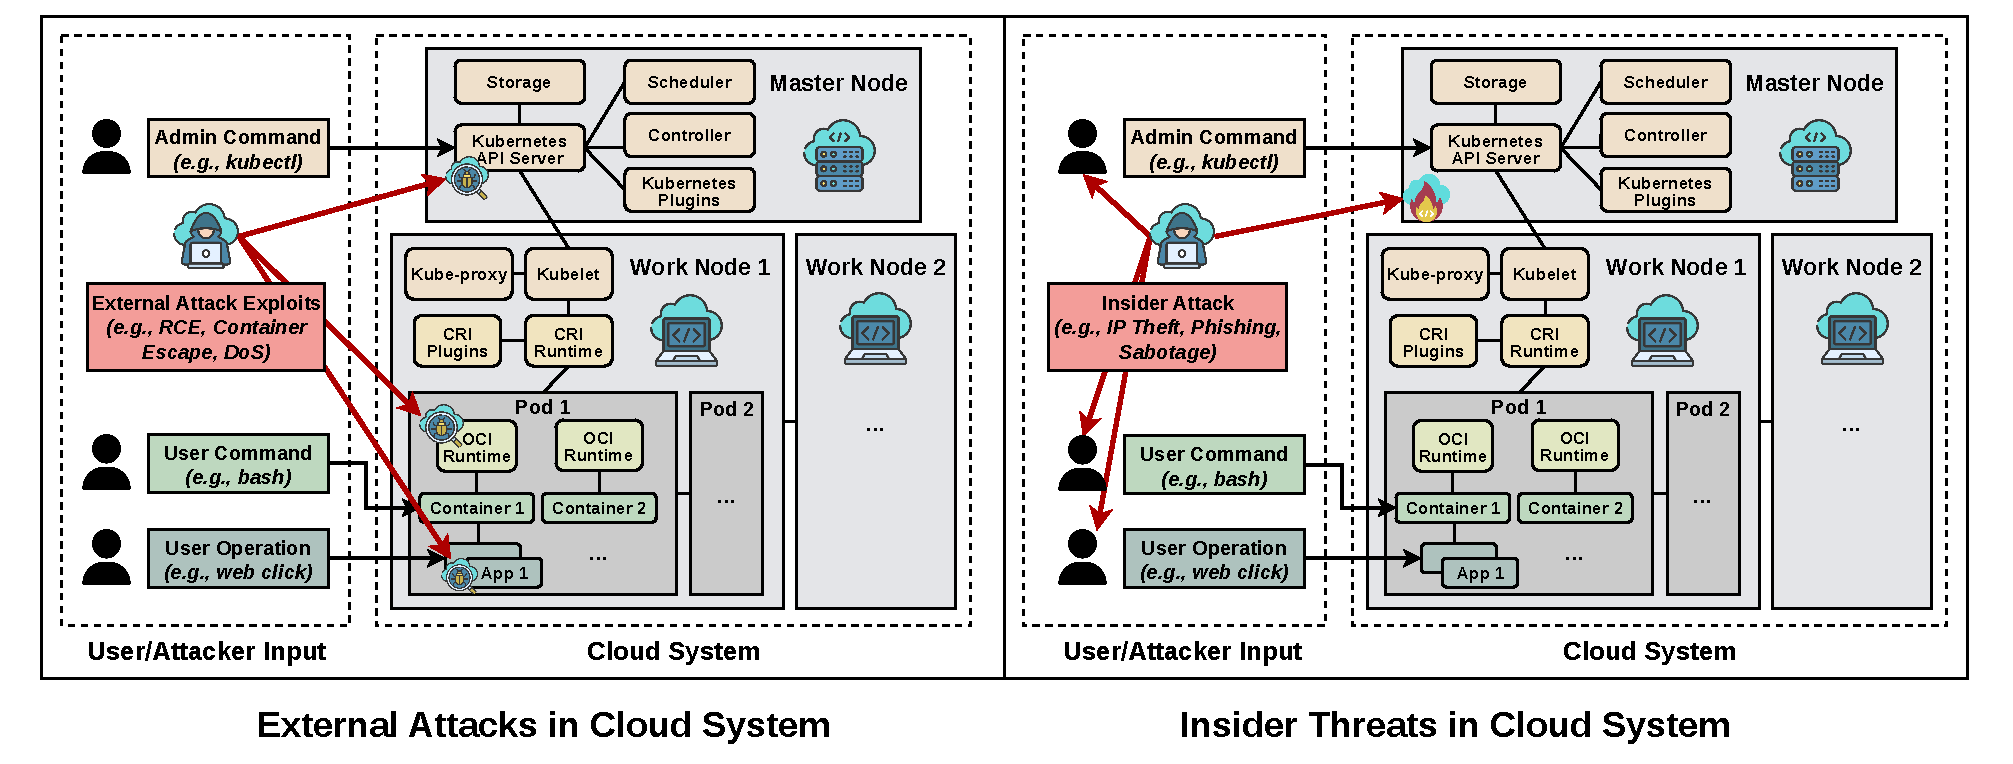
\includegraphics[width=1\linewidth]{Figures/Threats.pdf}
    \caption{Different threats in cloud systems.}
    \label{fig:attacksurface}
\end{figure}

\section{Limitations of Existing Approaches}

Despite extensive efforts to defend against the aforementioned threats, existing approaches primarily follow two directions: (1) securing cloud infrastructure through vulnerability detection and testing, and (2) detecting attacks via system-level monitoring and anomaly detection. However, these approaches exhibit fundamental limitations when applied to cloud-native environments:

\begin{itemize}
    \item \textbf{Lack of Systematic Understanding of Cloud Runtimes.} Existing studies mainly focus on identifying individual vulnerabilities, without a comprehensive understanding of defect patterns in critical cloud components such as container runtimes. Consequently, the characteristics and security implications of these defects remain underexplored, and the effectiveness of existing testing techniques is not well understood.

    \item \textbf{Limited Robustness of Attack Detection.} Most attack detection methods are developed under stationary assumptions, whereas cloud-native systems continuously evolve due to application updates, infrastructure changes, and configuration variations. Such dynamics introduce persistent distribution shifts, which can significantly degrade detection performance in practice.

    \item \textbf{Lack of Data for Insider Threat Analysis.} Insider threat detection is fundamentally constrained by the lack of realistic and high-fidelity data. Privacy and confidentiality restrictions limit access to real-world datasets, while existing public datasets fail to capture complex human-driven behaviors, hindering effective modeling and evaluation.
\end{itemize}

These limitations reveal a fundamental gap between existing security approaches and the dynamic, heterogeneous nature of cloud-native systems, motivating the need for more systematic and integrated solutions.

\section{Research Problems}

To bridge the above gaps, this dissertation advances the security of cloud-native systems along three complementary research directions:

\begin{itemize}
    \item \textbf{Defect Characterization in Cloud Runtimes.} This work investigates how to systematically characterize defect patterns in container runtime systems, analyze their root causes and security implications, and evaluate the effectiveness of existing testing techniques.

    \item \textbf{Robust Detection of External Attacks under Dynamic Environments.} This work studies how cloud-specific distribution shifts, induced by application evolution and infrastructure changes, affect detection performance, and explores shift-aware adaptation techniques (e.g., continual learning) to improve robustness.

    \item \textbf{Data-Driven Insider Threat Detection.} This work investigates how to systematically reenact insider threat scenarios and generate high-fidelity, behaviorally diverse data to enable more effective and generalizable detection.
\end{itemize}

\section{Overview of this Dissertation}

To address these research problems, this dissertation adopts a threat-driven and vertically integrated approach to cloud-native security, as illustrated in~\autoref{fig:thesis-overview}.

\begin{figure}[t]
\centering
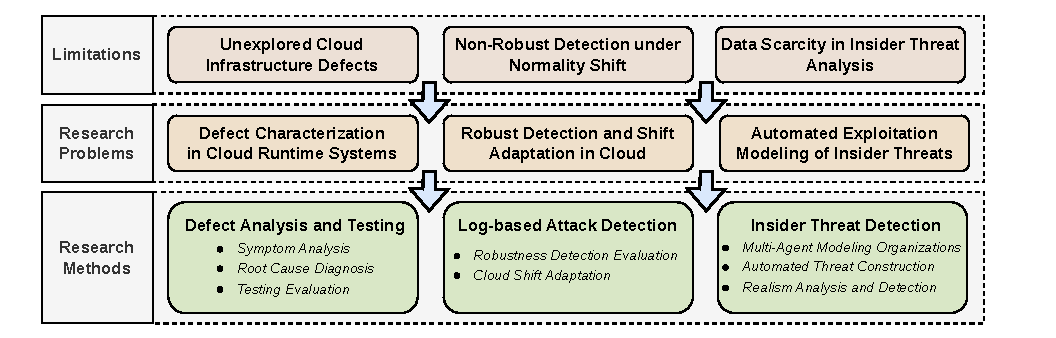
\includegraphics[width=1.0\textwidth]{Figures/Thesis-Overview.pdf}
\caption{{Overview of this dissertation.}}
\label{fig:thesis-overview}
\end{figure}

For real-world cloud-native systems, this dissertation investigates security challenges through a progressive perspective, moving from underlying software defects to externally observable attacks and, ultimately, to insider threats. First, it examines defects in critical cloud infrastructure components, particularly container runtime systems, with the goal of systematically characterizing defect patterns and understanding the limitations of existing testing techniques in detecting them. 

Second, building upon this foundation, it investigates the effectiveness of existing attack detection methods under dynamic system conditions when vulnerabilities are exploited by adversaries at runtime. In particular, it analyzes how evolving system behaviors, such as application updates and infrastructure changes, affect detection performance, and explores continual learning techniques to improve robustness in non-stationary environments. 

Finally, it addresses insider threat analysis within organizational boundaries. To overcome the lack of realistic data, it develops an LLM-based multi-agent framework that simulates organizational activities, generating both adversarial insider behaviors and behaviorally diverse, high-fidelity benign activities. This enables more generalizable insider threat analysis.

Through this progression, the dissertation integrates defect understanding, robust attack detection, and insider threat analysis into a unified and vertically structured framework for securing cloud-native systems.

\section{Main Contributions}

This dissertation makes the following key contributions:

\section{Publications}
The core of this dissertation is built upon the following first-authored research works:

\section{Dissertation Structure}

The remainder of this dissertation is organized as follows.

\chapter{Related Work}
\label{chap:related_work}

This chapter reviews prior research on cloud-native security from a problem-driven perspective aligned with this dissertation. We organize the literature along three interrelated dimensions: (1) security of cloud infrastructure software, (2) detection of external attacks in cloud environments, and (3) insider threat analysis. These dimensions reflect the fundamental sources of security risks in cloud-native systems, namely software defects, dynamic attack behaviors, and human-driven insider adversarial activities. For each dimension, we summarize representative approaches, analyze their underlying assumptions, and highlight their limitations in the context of modern cloud-native environments.

\chapter{Defect Characterization in CRS}

\section{Introduction}

Containers provide a highly flexible and portable solution for managing and deploying application workflows in the cloud. According to the Cloud Native Computing Foundation (CNCF) Annual Survey 2023~\cite{cncfannual}, containerization has become the predominant standard, with over 66\% of organizations adopting cloud native technologies in production. It highlights the benefit of widespread containerization and the ongoing shift towards a container-centric approach in cloud computing. As a result, ensuring the quality, reliability, and security of container infrastructure is paramount.

\chapter{Robust Attack Detection under Dynamic Cloud Environments}

\section{Introduction}

Cloud-native infrastructures featuring Kubernetes~\cite{k8s} and Docker~\cite{docker} have rapidly emerged as the predominant choice for modern cloud computing architectures, subsequently becoming the trending foundational infrastructure for hosting numerous software systems such as Software as a Service (SaaS) platforms. Existing studies report that Kubernetes has a commanding \textbf{92\%} market share among container orchestration tools used by businesses throughout the world~\cite{datadog-study} and over 50\% of Fortune-100 companies have adopted Kubernetes~\cite{oracle-study}. Despite the success, various security-critical attacks are key factors limiting the reliable use of cloud systems, such as the severe cloud vulnerability CVE-2024-21626~\cite{cve-2024-21626} that can result in container escape due to mishandling of file descriptor isolation. Therefore, ensuring the security of cloud systems is crucial. 

\chapter{Multi-Agent Simulation for Insider Threat Modeling}

\section{Introduction}

Insider threats refer to security incidents that originate from within an organization and have become a critical concern in modern enterprise environments. Recent studies report that over 50\% of organizations have experienced insider incidents, with 29\% incurring remediation costs exceeding one million dollars~\cite{ponemon2025insider,gurucul2024insider}. Detecting such threats remains particularly challenging as attackers are typically trusted insiders who possess legitimate access to organizational systems. Their malicious activities often blend into normal behavior and manifest in diverse forms, including horizontal propagation such as lateral movement within internal networks, unauthorized data exfiltration, IT sabotage, fraud, and espionage, as well as vertical escalation such as privilege escalation. Well-known incidents illustrate the severity of these threats, such as Edward Snowden's data exfiltration at the NSA~\cite{harding2014snowden} and employee-driven IT sabotage at Tesla in 2018~\cite{agnihotri2024tesla}. Traditional security defenses struggle to identify insider threats due to the legitimate access privileges of insiders, and this challenge is further exacerbated by inadequate monitoring infrastructure. Recent reports show that only 36\% of organizations have deployed comprehensive monitoring systems for proactive ITD~\cite{gurucul2024insider,signpost2025insider}, revealing significant gaps in current enterprise defenses.

\chapter{Conclusion and Future Work}

\section{Conclusion}

Cloud-native systems have become the foundation of modern software services, yet their security remains fundamentally challenged by software vulnerabilities in cloud infrastructure, external attacks under dynamic system behaviors, and human-driven insider adversarial activities. In cloud-native environments, external attacks may originate from exploitable software vulnerabilities and further evolve across multiple layers of the system, while insider threats arise from privileged or trusted entities operating within organizational boundaries. This dissertation improves the current understanding of these security problems through a progressive and threat-driven perspective, moving from infrastructure-level defect analysis to runtime attack detection and, ultimately, to insider threat analysis.

The main contributions of this dissertation are summarized as follows:

\begin{itemize}

\item \textbf{Defect Characterization in Cloud Infrastructure.} This dissertation presents a systematic empirical study of defects in container runtime systems. By analyzing real-world bugs, it identifies recurring defect symptom patterns and root causes, and reveals fundamental limitations of existing testing techniques in detecting these defects. These findings provide actionable insights for improving testing practices and reducing exploitable vulnerabilities in critical cloud components.

\item \textbf{Robust Detection of External Attacks under Dynamic Environments.} This dissertation investigates the effectiveness of log-based attack detection methods in non-stationary cloud environments. It introduces CAShift, a benchmark that models realistic system shifts caused by application updates, software evolution, and infrastructure changes. The results demonstrate significant performance degradation of existing methods under such conditions, and further provide a systematic adoption of continual learning strategies for shift adaptation, offering insights into their effectiveness in improving detection robustness under evolving system behaviors.

\item \textbf{Data-Driven Insider Threat Detection.} This dissertation proposes Chimera, an LLM-based multi-agent framework for simulating behaviorally diverse organizational activities. It models individuals as interactive agents to generate complex, human-driven behaviors. Based on this framework, it constructs ChimeraLog, a large-scale multi-modal dataset capturing both adversarial insider behaviors and high-fidelity benign activities. The generated data is validated through human expert evaluation and statistical analysis, demonstrating its realism and diversity, and highlighting the importance of data realism in enabling effective insider threat analysis.

\end{itemize}

\section{Future Work}

Building upon the findings of this dissertation, it identifies promising directions that can be explored to further advance the trustworthiness and security of cloud-native systems.

\bibliographystyle{plain}

\bibliography{thesis}
\end{document}
